\documentclass[12pt]{article}
\usepackage{amsmath}
\usepackage{amssymb}
\usepackage{tikz}
\usetikzlibrary{arrows.meta}
\usetikzlibrary{decorations.markings}

\begin{document}

\begin{figure}[h]
    \centering
    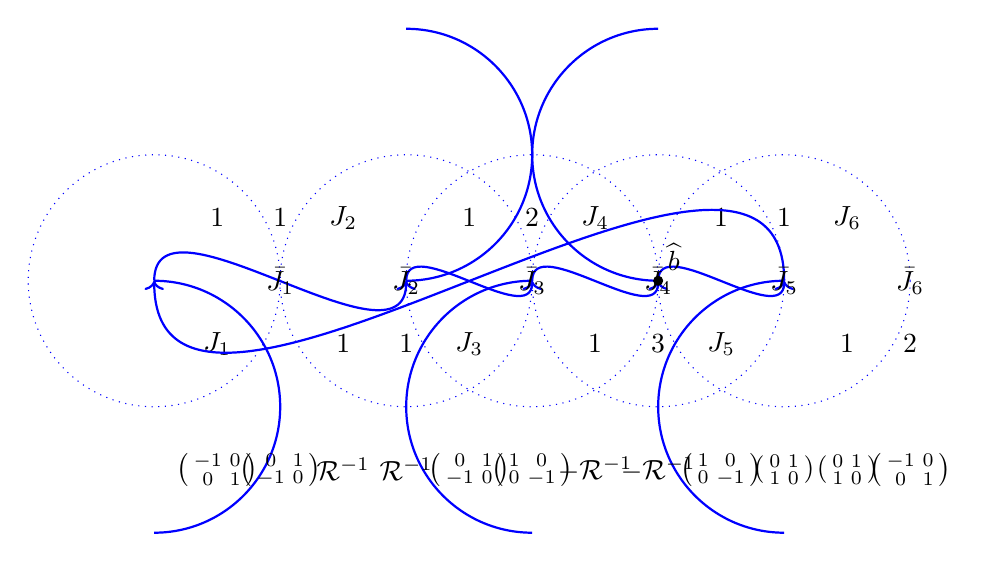
\begin{tikzpicture}[scale=0.8]
        % Define coordinates for the circles
        \coordinate (A) at (0,0);
        \coordinate (B) at (4,0);
        \coordinate (C) at (6,0);
        \coordinate (D) at (8,0);
        \coordinate (E) at (10,0);
        
        % Draw the circles
        \draw[blue,dotted] (A) circle (2cm);
        \draw[blue,dotted] (B) circle (2cm);
        \draw[blue,dotted] (C) circle (2cm);
        \draw[blue,dotted] (D) circle (2cm);
        \draw[blue,dotted] (E) circle (2cm);
        
        % Draw the arcs and labels
        \draw[blue,thick] (A) arc (90:-90:2cm);
        \draw[blue,thick] (B) arc (-90:90:2cm);
        \draw[blue,thick] (C) arc (90:270:2cm);
        \draw[blue,thick] (D) arc (270:90:2cm);
        \draw[blue,thick] (E) arc (90:270:2cm);
        
        % Label the arcs with J_i
        \node at (1,-1) {$J_1$};
        \node at (3,1) {$J_2$};
        \node at (5,-1) {$J_3$};
        \node at (7,1) {$J_4$};
        \node at (9,-1) {$J_5$};
        \node at (11,1) {$J_6$};
        
        % Label the sectors with 1
        \node at (1,1) {1};
        \node at (3,-1) {1};
        \node at (5,1) {1};
        \node at (7,-1) {1};
        \node at (9,1) {1};
        \node at (11,-1) {1};
        
        % Draw the matrix labels
        \node at (1,-3) {$\left(\begin{smallmatrix} -1 & 0 \\ 0 & 1 \end{smallmatrix}\right)$};
        \node at (3,-3) {$\mathcal{R}^{-1}$};
        \node at (5,-3) {$\left(\begin{smallmatrix} 0 & 1 \\ -1 & 0 \end{smallmatrix}\right)$};
        \node at (7,-3) {$-\mathcal{R}^{-1}$};
        \node at (9,-3) {$\left(\begin{smallmatrix} 1 & 0 \\ 0 & -1 \end{smallmatrix}\right)$};
        \node at (11,-3) {$\left(\begin{smallmatrix} 0 & 1 \\ 1 & 0 \end{smallmatrix}\right)$};
        
        % Draw the arrows for the strands
        \draw[->,blue,thick] (A) to[out=90,in=-90] (B);
        \draw[->,blue,thick] (B) to[out=90,in=-90] (C);
        \draw[->,blue,thick] (C) to[out=90,in=-90] (D);
        \draw[->,blue,thick] (D) to[out=90,in=-90] (E);
        \draw[->,blue,thick] (E) to[out=90,in=-90] (A);
        
        % Draw the labels for the strands
        \node at (2,0) {$\bar{J}_1$};
        \node at (4,0) {$\bar{J}_2$};
        \node at (6,0) {$\bar{J}_3$};
        \node at (8,0) {$\bar{J}_4$};
        \node at (10,0) {$\bar{J}_5$};
        \node at (12,0) {$\bar{J}_6$};
        
        % Draw the sector labels
        \node at (2,1) {1};
        \node at (4,-1) {1};
        \node at (6,1) {2};
        \node at (8,-1) {3};
        \node at (10,1) {1};
        \node at (12,-1) {2};
        
        % Draw the matrix labels
        \node at (2,-3) {$\left(\begin{smallmatrix} 0 & 1 \\ -1 & 0 \end{smallmatrix}\right)$};
        \node at (4,-3) {$\mathcal{R}^{-1}$};
        \node at (6,-3) {$\left(\begin{smallmatrix} 1 & 0 \\ 0 & -1 \end{smallmatrix}\right)$};
        \node at (8,-3) {$-\mathcal{R}^{-1}$};
        \node at (10,-3) {$\left(\begin{smallmatrix} 0 & 1 \\ 1 & 0 \end{smallmatrix}\right)$};
        \node at (12,-3) {$\left(\begin{smallmatrix} -1 & 0 \\ 0 & 1 \end{smallmatrix}\right)$};
        
        % Draw the basepoint
        \filldraw[black] (8,0) circle (2pt) node[above right] {$\widehat{b}$};
    \end{tikzpicture}
    \caption{Left: the formal local system before Fourier transform, Right: the formal local system after Fourier transform. The numbers in the circles show the identification of sectors given by Legendre transform. The green numbers show the numbering of the strands, given by choosing a numbering near a basepoint $\widehat{b}$ and continuing it compatibly in clockwise direction. The matrices are the partial formal monodromies given by the transformation rule (they come from the formal monodromies on the left, but change signs whenever one transits from a positive to a negative strand).}
    \label{fig:local_systems}
\end{figure}

\end{document}